\documentclass[../main/main.tex]{subfiles}

\newdate{date}{16}{10}{2020}


\begin{document}

\subsection{Usare il generatore per alimentare l'amplificatore}

Come si alimenta correttamente l'amplificatore in modo tale da essere sicuri di dare +12 V nel terminale positivo e -12 V nel negativo? Per fare questo bisogna collegare due alimentatori in serie e mettere il terminale in comune a massa (comune), come in Fig. \ref{fig:4_1}. Infatti in questo modo si è sicuri della differenza di potenziale che si sta dando a ciascun pin dell'amplificatore.

\marginpar{
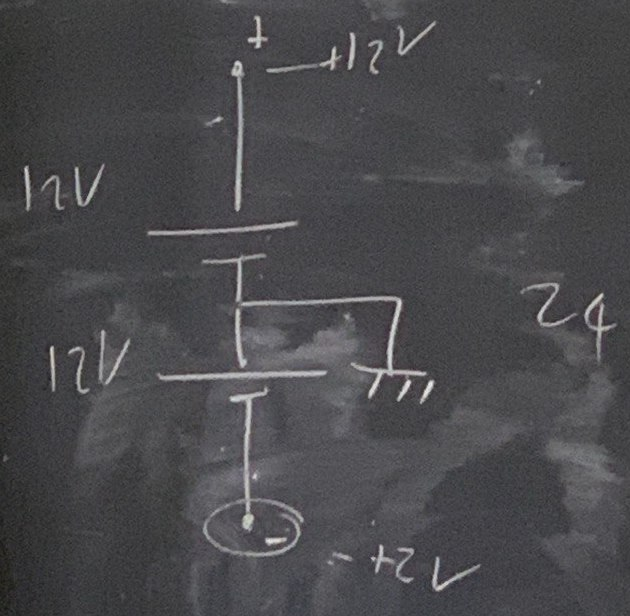
\includegraphics[width=\marginparwidth]{../lessons/image/04/1.jpg}
\captionof{figure}{\label{fig:4_1} Creare differenza di potenziale di 24 V connettendo in serie due generatori.}
}

\subsection{Assemblamento circuito}
Una volta capito come alimentare l'amplificatore, abbiamo assemblato il circuito come in Fig. \ref{fig:3_5}.


\marginpar{ \textbf{Laboratory 4.} \\  \displaydate{date}. \\ Compiled:  \today. }

\subsubsection{Circuito prova 1}
Per il primo circuito di prova abbiamo scelto alla fine:
\begin{itemize}
\item due condensatori da \( 1 \, \mu  \)F;
\item fissata una \( V_0 = 1\, V \);
\item presa una resistenza \( R_0 = 2.674 \,\text{k}\Omega  \);
\item presa \( R_{sc} = 11.2 \, \Omega  \);
\item presa \( R_G = 467.1 \, \Omega  \) che implica \( G = 108.04 \);
\item alimentato l'amplificatore con \( V_+ = 12 \) V e \( V_- = -12 \) V.
\end{itemize}
In questo modo ci aspettiamo che teoricamente:
\begin{equation*}
  V_{sc}^{th} = V_0 \frac{R_{sc}}{R_{sc}+R_0} = 4.171 \, \text{mV}, \qquad V_{out}^{th} = G V_{sc}^{th} = 450.649 \, \text{mV}
\end{equation*}
I valori misurati sono:
\begin{equation*}
   V_{out}^{mis} =  444.6 \, \text{mV}
\end{equation*}
Se invece utilizziamo \( V_0 = 0.5 \, \)mV (lasciando gli altri parametri invariati):
\begin{equation*}
   V_{out}^{th} =  225.32 \, \text{mV}, \qquad V_{out}^{mis} =  219.6 \, \text{mV}
\end{equation*}

\subsubsection{Circuito prova 2}
Per il secondo circuito di prova abbiamo scelto:
\begin{itemize}
\item due condensatori da \( 1 \, \mu  \)F;
\item fissata una \( V_0 = 0.5 \, \)V;
\item presa una resistenza \( R_0 = 21.83 \,\text{k}\Omega  \);
\item presa \( R_{sc} = 11.2 \, \Omega  \);
\item presa \( R_G = 98.5 \, \Omega  \) che implica \( G = 508.614 \);
\item alimentato l'amplificatore con \( V_+ = 12 \) V e \( V_- = -12 \) V.
\end{itemize}
In questo modo ci aspettiamo che teoricamente:
\begin{equation*}
  V_{sc}^{th} = 0.2564 \, \text{mV}, \qquad V_{out}^{th} = 130.4 \, \text{mV}
\end{equation*}
I valori misurati sono:
\begin{equation*}
   V_{out}^{mis} =  125.2 \, \text{mV}
\end{equation*}
anche se si nota come utilizzando un'amplificazione maggiore il valore di tensione misurato oscilli maggiormente (utilizzando il multimetro).

\subsubsection{Circuito finale 1}
Per il circuito finale abbiamo scelto:
\begin{itemize}
\item due condensatori da \( 1 \, \mu  \)F;
\item fissata una \( V_0 = 0.5 \, \)V;
\item presa una resistenza \( R_0 = 220.1 \,\Omega  \);
\item presa \( R_{sc} = 0.3 \, \Omega  \);
\item presa \( R_G = 98.5 \, \Omega  \) che implica \( G = 508.614 \);
\item alimentato l'amplificatore con \( V_+ = 12 \) V e \( V_- = -12 \) V.
\end{itemize}
In particolare, per la \( R_{sc} \) abbiamo utilizzato il nostro superconduttore. Il valore è stato misurato con il multimetro che non ci darà mai una stima affidabile in quanto di default tra i due terminali del multimetro si misurano comunque circa \( 0.2 \, \Omega  \). Proprio per l'incapacità stessa di misurare la resistenza con il multimetro, stiamo realizzando questo circuito con l'amplificatore.

Con i parametri sopra stabiliti, ci aspettiamo che teoricamente:
\begin{equation*}
  V_{sc}^{th} = 0.74887 \, \text{mV}, \qquad V_{out}^{th} = 380.886 \, \text{mV}
\end{equation*}
Si misura che:
\begin{equation*}
   V_{out}^{mis} =  332 \, \text{mV}
\end{equation*}
Il discostamento dal valore teorico è abbastanza, ma non esageratamente grande. Questo è dato dal fatto che magari la resistenza del nostro superconduttore non sia davvero di \( R_{sc} = 0.3 \, \Omega  \), ma inferiore.

Invece utilizzando \( R_G = 467.1 \, \Omega  \) (\( G = 108.04 \)), si misura:
\begin{equation*}
   V_{out}^{th} =  80.9079 \, \text{mV}, \qquad V_{out}^{mis} =  56.5 \, \text{mV}, \quad V_{sc}^{mis} = 0.5229 \, \text{mV}
\end{equation*}
Facendo il calcolo inverso otteniamo che:
\begin{equation*}
  R_{sc}^{mis} = \frac{V_{sc}^{mis}}{I} = V_{sc}^{mis} \frac{R_0}{V_0} = 0.23 \, \Omega
\end{equation*}
Questo calcolo è un po' tautologico però ci permette di capire la differenza nelle misurazioni a cosa può essere dovuta.

Il circuito finale è mostrato in Fig. \ref{fig:4_2} e in Fig. \ref{fig:4_3}.

\begin{remind}{}{}
    Prima di accendere il circuito, è importante controllare che la potenza dissipata deve essere minore del mW, se no il superconduttore si autoriscalderà e non riusciremo a misurare realmente la temperatura critica. Notiamo che con questi valori di resistenze e potenziali la condizione è soddisfatta:
    \begin{equation*}
      P_{sc}^{dissipata} = \frac{V_{sc}^2}{R_{sc}} = 1.87 \times 10^{-6} W
    \end{equation*}
\end{remind}


\begin{figure}[h!]
\centering
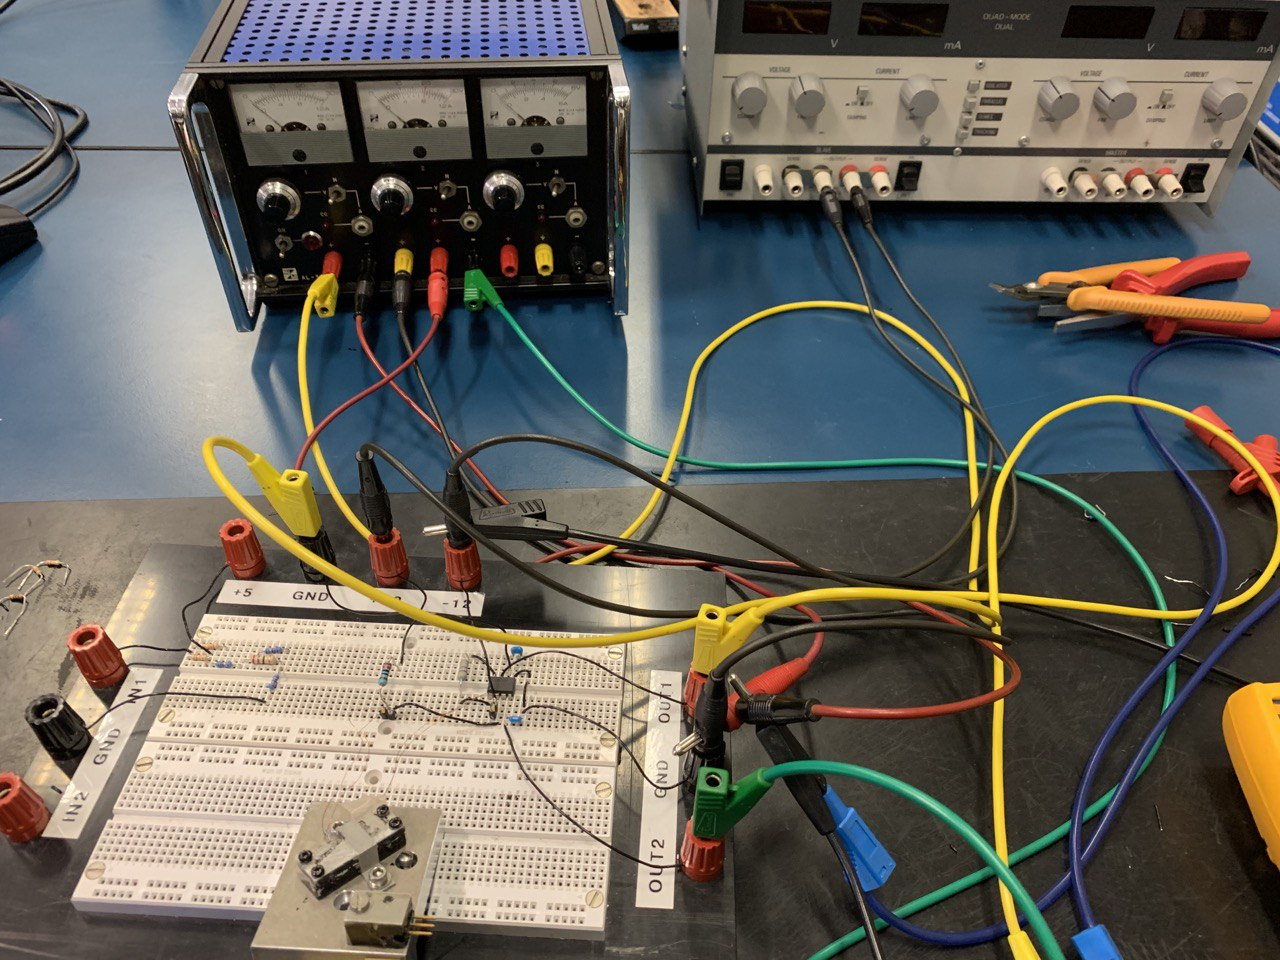
\includegraphics[width=0.7\textwidth]{../lessons/image/04/2.jpg}
\caption{\label{fig:4_2} Circuito finale.}
\end{figure}

\begin{figure}[h!]
\centering
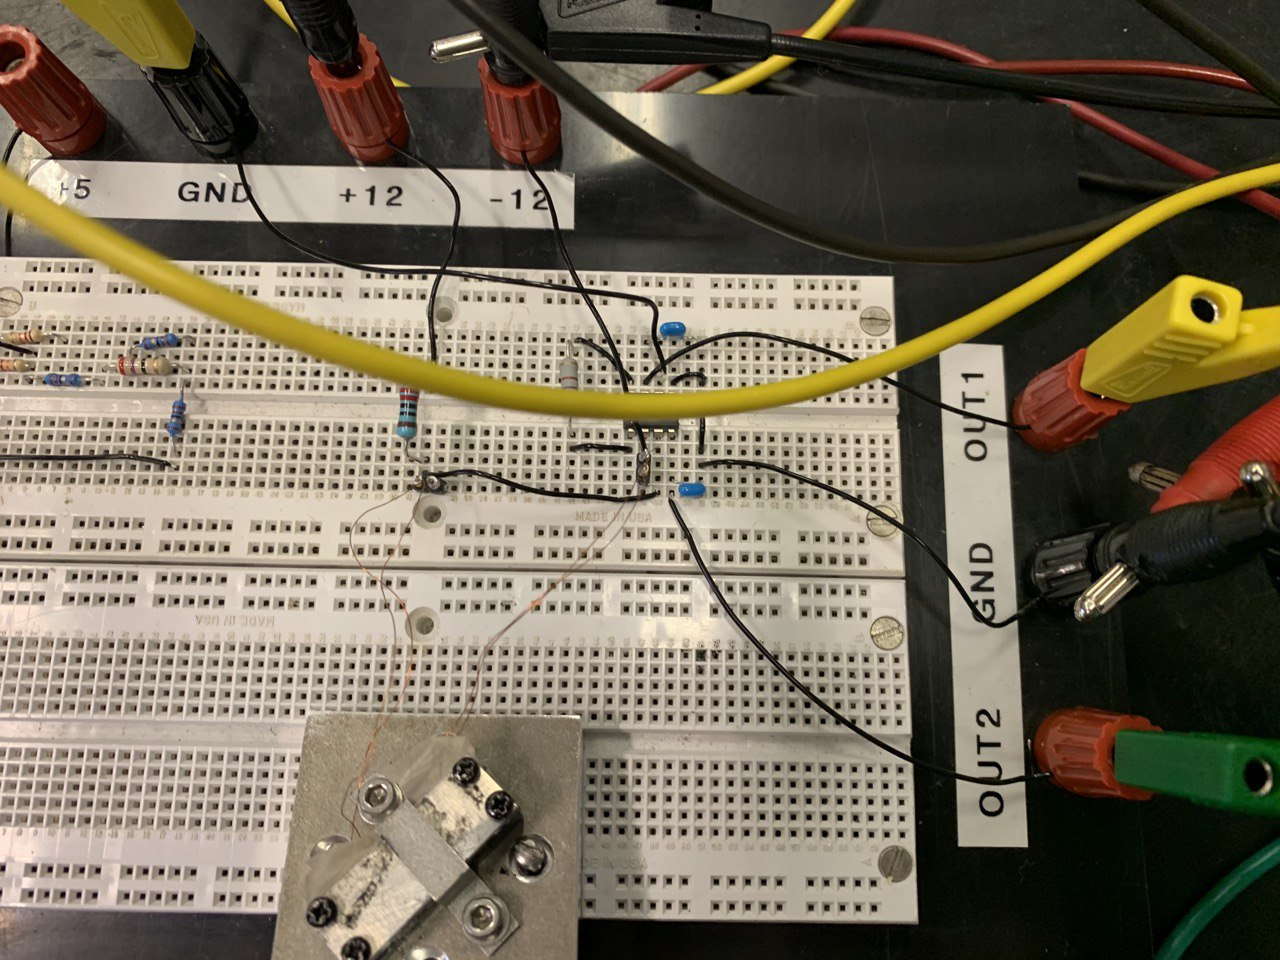
\includegraphics[width=0.7\textwidth]{../lessons/image/04/3.jpg}
\caption{\label{fig:4_3} Circuito finale (altra angolazione).}
\end{figure}

\end{document}
